% !TEX TS-program = xelatex
% !TEX encoding = UTF-8 Unicode

\providecommand{\home}{../..}
\documentclass[\home/main.tex]{subfiles}

\begin{document}

\chapter{Learning reward functions from demonstrations}\label{ch:reward_functions}
% Doel: Beschrijf de hele pipeline, high-level en toegankelijk

% High-level en concreet: welk probleem los je op?

We define the problem of using multi-perspective images with task or demonstrations to construct a metric that indicates the task progression and solution quality. We want the task progression metric to increase on important moments when progression is made towards solving the task. Central in our framework is (1) the generation of a meaningful semantic embedding that indicates task progression and solution quality and (2) mapping this embedding to a scalar value. A high-level overview is given in Figure~\ref{fig:overview}. Our method consists of three main steps. First, we use multi-perspective video frames to train an embedding using contrastive learning. This is done by using time as a self-supervisory signal. This method allows to learn useful invariances and forces the network to focus on task-relevant properties as we will show in Section~\ref{sec:results}. We take a small sample of the demonstrations which we label \textit{experts} as they will be used as a reference for indicating task progression. Second, we align the embeddings of the demonstrations to the task executions of experts using dynamic time warping. Third, we use this alignment to query the ensemble of experts for predicting task progress.

% Hier komt de high-level overview figuur, gedefinieerd in tex code 
\pgfdeclarelayer{edgelayer}
\pgfdeclarelayer{nodelayer}
\pgfdeclarelayer{subnodelayer}

\pgfsetlayers{edgelayer,nodelayer,subnodelayer,main}
\tikzstyle{block} = [rectangle, draw, fill=blue!20, text width=17.5em, text centered, rounded corners, minimum height=2em]
\tikzstyle{embed_block} = [rectangle, draw, fill=blue!40, text width=5em, text centered, minimum height=1em]

\tikzstyle{dataset} = [cylinder, draw,  shape border rotate=90, fill=blue!20, text width=2.5cm, text centered, rounded corners, minimum height=1cm,minimum width=1cm, shape aspect=.5]

\tikzstyle{line} = [draw, -latex']
\begin{figure}[htbp!]
\centering

\begin{tikzpicture}[node distance = 2cm, auto]
  	\begin{pgfonlayer}{nodelayer}
  	
	\node [dataset] (video_data) {Video task demonstrations};	

	\node [block, right of=video_data, node distance=7cm] (tcn) {\nameref{subsec:tcn} \footnotesize{(section \ref{subsec:tcn})}};
	\node [block, below of=tcn] (dtw) {\nameref{subsec:dtw} \footnotesize{(section \ref{subsec:dtw})}};
	\node [block, below of=dtw] (extract) {\nameref{subsec:extract} \footnotesize{(section \ref{subsec:extract})}};

    \end{pgfonlayer}
        
   	\begin{pgfonlayer}{edgelayer}

	\path [line, dashed] (video_data) -- node{all samples}(tcn);
	\path [line, dashed, latex'-] (dtw) -| node[text width=2cm]{High-quality samples only}(video_data);
	\draw[line, dashed, -latex'] (0,-2) |- (extract); %\path [line, dashed, latex'-] (extract) -| node{}(video_data);
	
	\path [line, thick] (tcn) -- (dtw);
	\path [line, thick] (dtw) -- (extract);

    \end{pgfonlayer}
\end{tikzpicture}

\caption{{\textbf{High-level overview of our methodology.}}}
\label{fig:overview}
\end{figure}

Our method assumes the availability of task demonstrations with corresponding process metrics. The demonstrations can range from teleoperated machinery to sensor recordings external to the executing body. We focus in particular on using recorded process metrics in the form of multi-perspective camera streams. Our method is deployable for arbitrary processes and tasks for which example demonstrations are available. These demonstrations are allowed to contain sub-par solution strategies. The method requires selecting a small part of the data, in our experiments $5\%$, as a reference for a good task solution. We focus on task demonstrations given by humans, but any entity solving the task can be used as input. Our methodology is applicable in settings where process monitoring is essential for output quality. We exploit temporal coherence which requires the process to contain measurable inputs along a temporal dimension.
For example, multiple cameras filming how human workers are sewing the front and back of a shirt together.
Another major application we target is learning of robotic manipulation skills using RL. This is because the field of RL heavily borrows the concept of expressing task progression and solution quality in a scalar value called the reward function. This reward function is used to learn an agent to solve a designated task in an unknown environment. Engineering such reward functions is difficult for some domains like folding clothing and autonomous driving. Our method allows learning a reward function without supervision, which can be used downstream for a learning agent requiring supervision in the form of a scalar value expressing task progression.

\section{Methodology for unsupervised learning of reward functions}\label{sec:methodology}
\subsection{Learning semantic meaningful embeddings using TCNs}\label{subsec:tcn}
Central in the proposed framework is learning task-relevant representations containing the notion of task progression and solution quality. We use \acrfullpl{TCN}~\cite{Sermanet2017TCN} in which time serves as a supervisory signal. \acrshortpl{TCN} are a self-supervised method for training abstract representations of the progression of a task. The core concept is to push video frames distant in time away and pull them together when they are near in time. Multiple cameras are used to capture several perspectives of the same demonstration in a synchronized manner. This principle is shown in Figure~\ref{fig:triplet_mining}. Any pair of frames from different camera angles that occurred at the same time must be close together in embedding space. Frames from the same camera angle that are separated by time are forced to be distant in embedding space. This principle encourages the network to attend to high-level features relevant for the task.
Attending to irrelevant background noise or low-level features would attract negative pairs from the same perspective and repulse positive pairs from different perspectives. This way, the correspondence problem~\cite{BrassHeyes2005} for imitation learning can be solved. In case the network tries to explain the visual difference between two temporal distant frames by looking at the demonstrator, it would pull the anchor and negative close together, leading to a higher loss. The only way to achieve a lower loss is by looking at task-relevant features: what is consistently changing in the scene that cannot be attributed to changes in viewpoint, lighting, occlusion, and background.

% Formele uitleg en triplet mining 
Formally, if the embedding of an input is given by $f(x) \in \mathbb{R}^d$, we can then define the loss between an anchor $x_i^a$, positive $x_i^p$ and negative frame $x_i^n$ as~\cite{FaceNet}:
\begin{align}
    \left\|f\left(x_{i}^{a}\right)-f\left(x_{i}^{p}\right)\right\|_{2}^{2}+\alpha<\left\|f\left(x_{i}^{a}\right)-f\left(x_{i}^{n}\right)\right\|_{2}^{2} \nonumber, \\
    \forall\left(f\left(x_{i}^{a}\right), f\left(x_{i}^{p}\right), f\left(x_{i}^{n}\right)\right) \in \mathcal{T},    \nonumber
\end{align}
with $\alpha$ being the margin enforced between positive and negative pairs. $\mathcal{T}$ represents all possible triplets, i.e. all \textit{anchor-positive-negative} combinations. The loss we are trying to minimize then becomes:
\begin{equation*}
    \sum_{i}^{N}\left[\left\|f\left(x_{i}^{a}\right)-f\left(x_{i}^{p}\right)\right\|_{2}^{2}-\left\|f\left(x_{i}^{a}\right)-f\left(x_{i}^{n}\right)\right\|_{2}^{2}+\alpha\right]_{+}.
\end{equation*}

%To gather the triplets $\mathcal{T}$, we use a semi-hard triplet mining strategy~\cite{FaceNet}. This guides the training process to focus on increasingly harder anchor-positive-negative pairs. For every batch, we mine triplets online by starting to sample pairs of \textit{(anchor, positive)} such that no other sample in the batch is a positive to the anchor frame. By extension, all other samples in the batch are negatives to that anchor sample. After the forward pass through the network, a distance matrix is computed between all embeddings in the batch. We aim for a scenario in which the distance between the anchor embedding and all negative embeddings is equal to or greater than the distance between the anchor and positive embeddings, incremented by a small margin. Any \textit{anchor, negative} pair that does not meet this criterion is considered an easy triplet and removed from the batch. The loss score for one anchor is defined as the difference between the \textit{anchor, positive} distance plus margin (i.e., the desired minimal distance) and the greatest \textit{anchor, negative} distance among the fail pairs (i.e., the fail case that is closest to the desired minimal distance). This process can be seen as pushing the fail-cases out of the minimal distance range one-by-one, starting with the easiest. 

%TODO: Tekst strakker zetten en meer naar volgende verwerken: We minen naar semi-hard triplets. We doen dit door random frames %met willekeurige perspectieven te samplen. Voor ieder anchor definieren we positives als binnen een tijdsrange van t frames. %Dit is een hyperparam. We selecteren tijdens training per anchor het moeilijkste positive = waar afstand(anchor, pos) het %grootste is. Voor deze anchor-positive pairs zoeken we het gemakkelijkste semihard. Semihard = afstand tussen anchor-pos is %kleiner dan anchor-neg maar afstand anchor-neg is kleiner dan anchor-pos plus een marge. Indien er geen semihards zijn, nemen %het gemakkelijkste hard (i.e. waar afstand anchor-pos groter is dan anchor-neg). Als deze niet zou bestaan, nemen we de %moeilijkste easy negative. Dit is een batch hard principle uit citep{In Defense of the Triplet Loss for Person %Re-Identification}. Intuitief komt dit overeen met "as pushing the fail-cases out of the minimal distance range one-by-one, %starting with the easiest".
%
%We kunnen hier ook een figuur toevoegen:
%            A --------- P ------------- m ---------------------
%                HARD SEMI-HARD EASY

To gather the triplets $\mathcal{T}$, we use a semi-hard triplet mining strategy with an increasing difficulty level. The goal of this strategy is to guide the training process to focus on increasingly harder \textit{anchor-positive-negative} triplets. We do this by first sampling random anchors and positive frames from all possible perspectives. Positive frames are defined as temporal neighbours that are at a maximum $\epsilon$ frames sampled around the anchor. Frames further away are labelled as negatives. This principle is visible in Figure~\ref{fig:triplet_mining}. For each anchor during training, we select the most difficult positive, i.e., where the distance between the anchor and positive is the largest. For this \textit{anchor-positive} pair, we calculate the distance between the semi-hard negatives and anchor. Semi-hard negatives are defined as contrastive samples to the anchor which are of reasonable difficulty: the distance between \textit{anchor-negative} pair is marginally larger than the distance between the \textit{anchor-positive} pair. Intuitively, this corresponds with pushing the fail-cases out of the minimal distance range one by one, starting with the easiest. We define the cost function of the batch as the average loss scores overall anchor frames.

\begin{figure}[htbp]
    \centering
    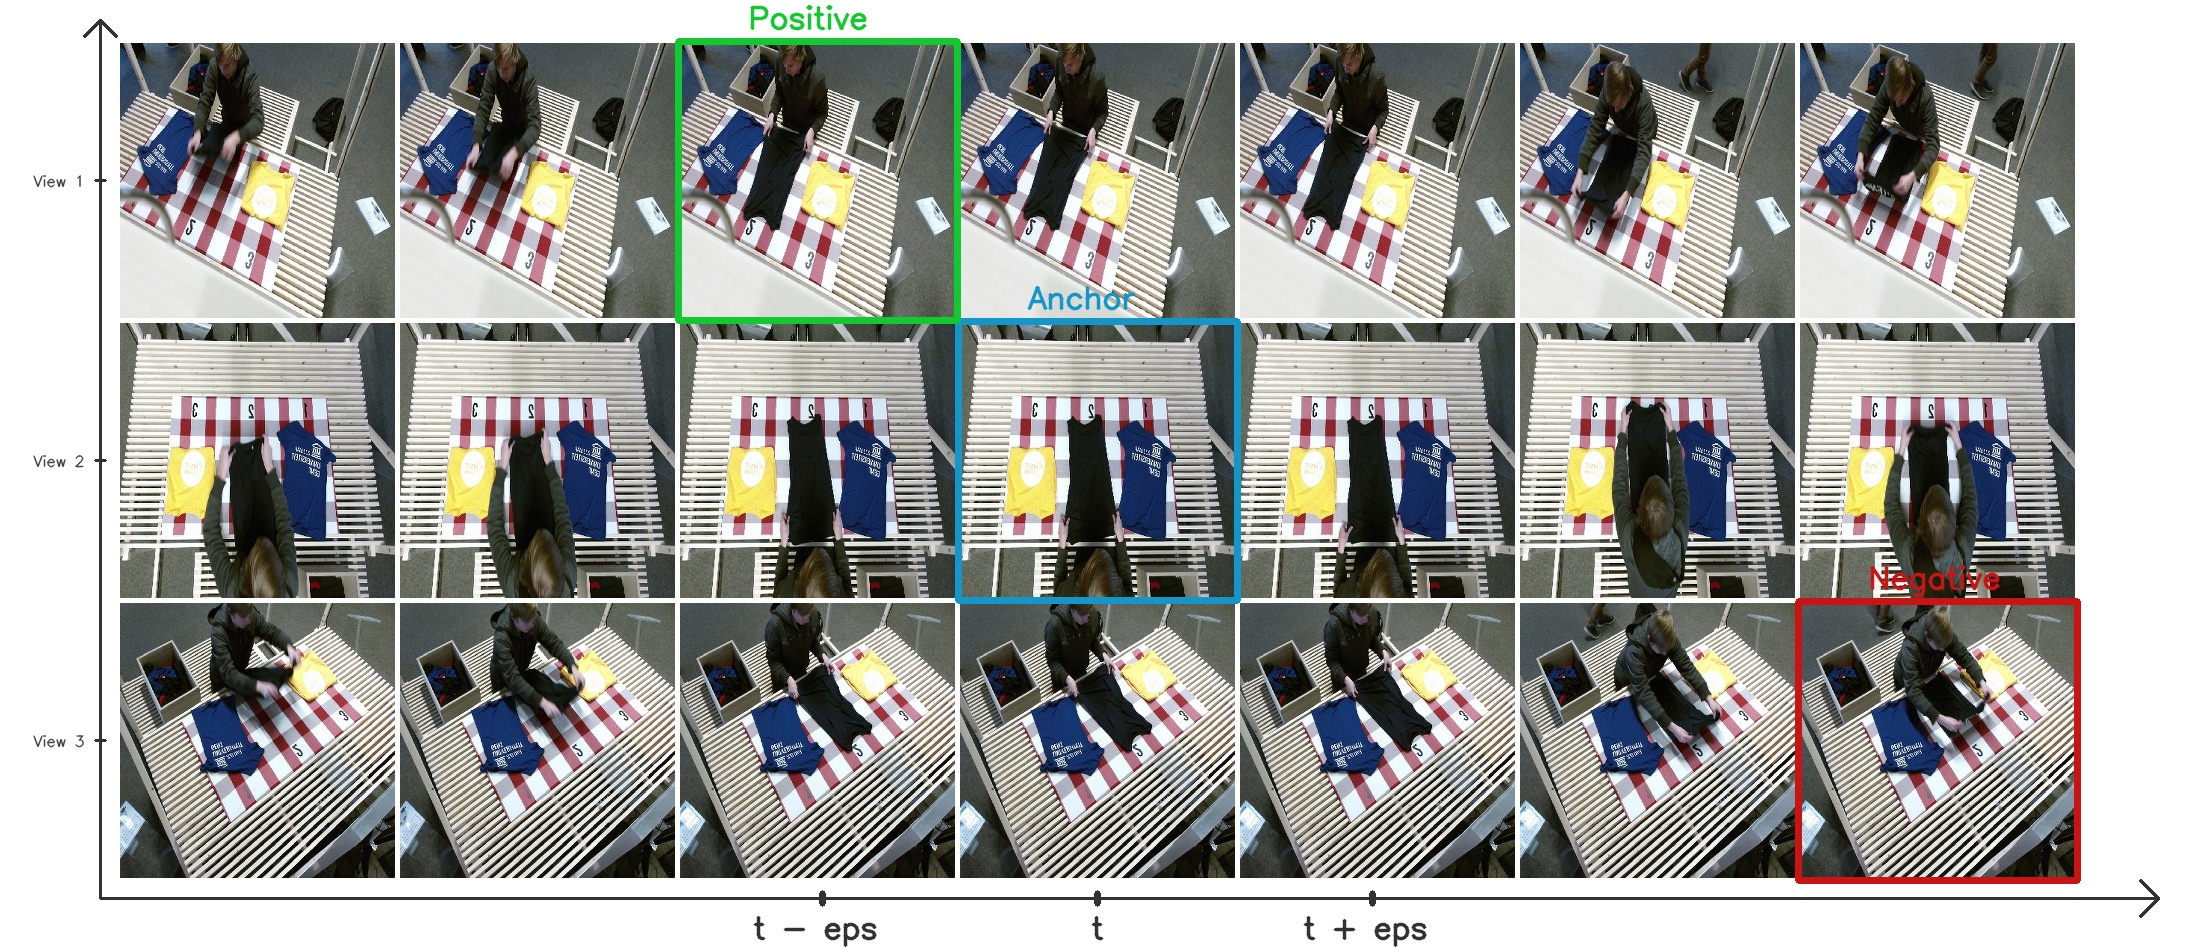
\includegraphics[width=0.90\textwidth, keepaspectratio]{\home/chapters/05-reward_functions/figures/figs_tcn_sampling.jpg}
    \caption{\textbf{Using time as a supervisory signal in \acrshortpl{TCN}}. A randomly selected anchor frame (in blue) and a nearby temporal neighbor from a different perspective (in green) are encouraged to be close in the embedding space compared to the anchor frame and a distant temporal neighbor (in red). This allows the network to learn to explain changes in the physical world.}
    \label{fig:triplet_mining}
\end{figure}

\subsection{Aligning expert video embeddings with query videos} \label{subsec:dtw}

% Structuur: 
%   Waarom DTW nodig, wat komt er in
%   Hoe werkt oorspronkelijk DTW -> grijp terug naar referentiewerk
%   Beschrijf aanpassingen dat we doen: move backwards in time + check impl

The TCN embedding trained in the previous Section~\ref{subsec:tcn} gives rise to a multivariate time series. In order to compare the time series embedding of a demonstrator $X = (x_1, \ldots, x_i, \ldots, x_N)$ to that of a chosen expert $Y = (y_1, \ldots, y_i \ldots, y_M)$ in order to judge the quality of the folding demonstration. To calculate the alignment between these time series, we use \acrfull{DTW}~\cite{Bellman1959}. \acrshort{DTW} is an algorithm for measuring the similarity between time series under time distortions. It minimizes the effects of shifting in time by allowing elastic transformations of the time series, subject to time-normalization constraints. This allows accounting for nonlinear task execution rate differences between two demonstrations. In \acrshort{DTW} , an optimal path $P^*$ mapping time series $X$ and $Y$ are found:

% This is the previous notation where the time index was a subscript instead of variable
%\begin{align}
%    P^* = \argmin_{\phi_t, \psi_t} \sum_{t=1}^{\text{T}} d(x_{\phi_t}, y_{\psi_t}) \\
%\end{align}

\begin{subequations}
\begin{alignat}{2}
&\!P^* = \argmin_{\phi_x, \phi_y}        &\qquad& \sum_{t=1}^{\text{T}} d(x_{\phi_x(t)}, y_{\phi_y(t)}),\nonumber\label{eq:of}
%\\ TODO: we kunnen opteren om deze constraints voluit te schrijven
%&\text{subject to} &      & \phi_x(1)=1,\nonumber\\
%&                  &      & \phi_y(1)=1,\label{eq:startpoint}\\
%&                  &      & \phi_x(T)=N,\nonumber\\
%&                  &      & \phi_y(T)=M,\label{eq:endpoint}\\
\end{alignat}
\end{subequations}
with $d()$ being a local distance function, for example, Euclidean distance. The alignment between the two time series is established through the mapping functions $(\phi_x(t), \phi_y(t))$. The warping functions are limited by certain constraints in order to be meaningful. Common warping constraints~\cite{Rabiner1993} are (1) start- and endpoint constraints as a clear start and end are manually specified by preprocessing the data, (2) monotonicity constraint which maintains temporal order during time normalization, and (3) local continuity constraints, also known as step patterns, to minimize loss of information. Compared to the canonical version of \acrshort{DTW}, we relax the monotonicity constraint, which specifies that the alignment path does not go back in time. By allowing the time index of the expert time series $Y$ (i.e., the reference signal) to go back in time, we can account for demonstrators restarting part of the task execution or even executing the task backward. This also allows for coping with a failed task execution. We also relax the formulation to open-end \acrshort{DTW}~\cite{Tormene2009} by removing the endpoint constraint to incorporate the possibility that demonstrators are not finishing the task optimally or completely. A visual interpretation on how we align a demonstration to video frames of an expert is given in Figure~\ref{fig:dtw}. We show the single component of two fictitious one-dimensional embeddings. The demonstration of which we need to calculate the task progression is labeled as the query. This is aligned to the embedding time series of the expert. The warping path is drawn in the global cost matrix. The colored sections on the time series and alignment path represent subtasks. The background colors represent similar task progression or the same subtasks in the videos of the expert and query sample.  

\begin{figure}[htbp]
    \centering
    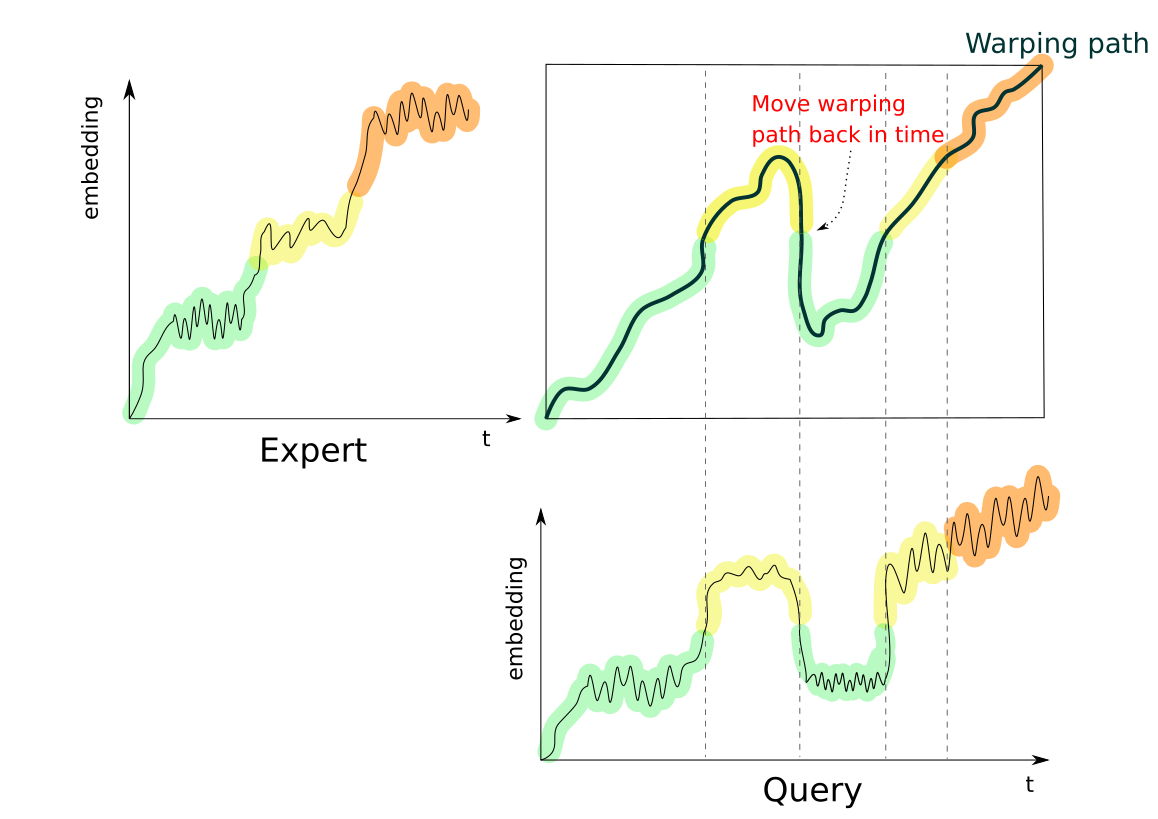
\includegraphics[width=0.90\textwidth, keepaspectratio]{\home/chapters/05-reward_functions/figures/figs_dtw_backwards_v05.png}
    \caption{\textbf{Dynamic Time Warping (DTW) without monotonicity constraint.} We align a multivariate time series embedding of a demonstration (the query) to the video frames of an expert. The time index is allowed to go back in time so we can align correctly in case a demonstration reverses some of the executed actions.}
    \label{fig:dtw}
\end{figure}

\subsection{Extracting task progression from embeddings} \label{subsec:extract}
The last step in our methodology is to extract task progression indicators using the aligned embeddings. First, we search which frame of each expert aligns best with each frame of the demonstration. The alignment score is expressed as the reciprocal of the cost of the best fit between them. Then, we select the temporal index of the best matching frame of every expert and express it as progress in percentage. Next, we average the experts' progress ratings by weighting with the normalized fit scores of the DTW phase of the pipeline. Finally, we remove any outliers by rejecting progress predictions of experts that deviate too much from the median of the absolute deviations~\cite{Leys2013}. %$\frac{X_i - \text{median}(X)}{b ~\text{median}(\left |X_i - \text{median}(X)  \right |)}$

%\begin{figure}[htbp]
%    \centering
%    \includegraphics[width=0.90\textwidth, keepaspectratio]{figures/reward function calculation.jpg}
%    \caption{We calculate the reward for each demonstration frame by querying the temporal location of the %aligned frames of the experts.}
%    \label{fig:reward_fuction_calc}
%\end{figure}



\section{Results on folding clothing}\label{sec:results}
% GOAL: describe what comes out of the proposed framework = data collection, result of TCN training, result of reward extraction 

% Content: What is the task, why is this relevant, how did we do it, what does the data look like

We apply our methodology to the challenging case of assessing the task progression and quality of folding clothing. Manipulation of clothing and other deformable objects is considerably harder compared to rigid object manipulation due to the infinite amount of configurations the object can be in. This makes the domain of deformable object manipulation relevant for our application: state estimation is very difficult given the deformations exercised on the clothing~\cite{Foresti2004}. In order to assess the quality of the executed manipulations, it is necessary to estimate how well the clothing is folded by identifying the final shape and detecting wrinkles. Performing this state estimation manually is time-consuming. Automated annotation processes rely on extracting contours of the textile using color segmentation~\cite{Miller2012}, utilizing depth camera's to detect wrinkles~\cite{Doumanoglou2016} and equipping the textile with tactile sensors~\cite{Verleysen2020-folding}. However, these methods do not scale and generalize well as they require prior information about the state of the clothing and considerable engineering effort. In contrast, asking people to give folding demonstrations is a cost-efficient way to gather data. 

In the remainder of this section, we present experimental results of applying our framework to extract task progression metrics based on video demonstrations of humans folding clothing. We first describe how we crowd-sourced human folding demonstrations, followed by a quantitative analysis of the learned embeddings of these video demonstrations. We conclude by qualitatively examining the resulting task progression metrics functions on a test set. 

\subsection{Folding demonstration dataset}
\subsection{Training results}
\subsection{Reward function results}

\section{Discussion}
\subsection{Semantic meaning of learned TCN embeddings {\tiny UMAP + clustering}}
\subsection{Case-based examples for post hoc interpretability}

\section{\textsc{[optional]} Results on folding clothing in simulation {\tiny claim van reward function testen}}
\subsection{Dataset generation}
\subsection{Resulting reward functions on simulated cloth}
\subsection{Learning to fold with unsupervised reward functions}

\section{Conclusion}

\end{document}